% !TEX root = ../thesis.tex

\chapter{Vyhodnotenie vytvoreného crawlera}
\label{evaluation}

% Vyhodnocovacia časť je kľúčovou časťou záverečnej práce. Tato časť obsahuje vyhodnotenie navrhnutého (vytvoreného) riešenia. Uprednostňované je objektívne vyhodnotenie výsledkov práce, ktoré sa opiera o~meranie a štatistické metódy, prípadne matematické dôkazy. V~prípade nameraných hodnôt musí autor opísať metódu merania, priebeh merania, výsledky a interpretáciu výsledkov v~kontexte riešeného problému a stanovených cieľov. Na základe vyhodnotenia riešenia autor opíše prínosy svojej práce. Vyhodnocovacia časť tvorí zvyčajne ¼ jadra práce.

Pre demonštráciu funkčnosti nášho riešenia sme ho nasadili na 11 hodín a zozbierali štatistiky z jeho behu popísané v kapitole \ref{c:collectingStats} . Ich vyhodnotením rozhodneme, či riešenie je vhodné na plánovanú prevádzku. Taktiež rozhodneme v akej miere sa nám podarilo splniť stanovené požiadavky.

Crawler sme navrhli na dlhodobú prevádzku. Preto sme sa vyhli zväčšujúcim sa dátovým štruktúram. Teda veľkosť využitej pamäte je v čase takmer konštantná. Urobili sme výnimku pre Url manažér modul. Najprv sme plánovali ho implementovať pomocou databázového systému ale pre splnenie požiadavky na nízku komplexitu sme skúsili jednoduchšiu implementáciu a potrebné informácie držíme priamo v operačnej pamäti. Teda s rastúcim prevádzkovým časom rastú aj pamäťové nároky. V kapitole \ref{c:perfDegr} vyhodnotíme, či tento prístup je vhodný pre dlhšie prevádzky a teda či toto rozhodnutie bolo správne. 


\section{Popis nasadenia}
Crawler sme spúšťali dňa 13.5.2023 o 20:00 na 11 hodín. Nastavenia a špecifikácie systému na ktorom bežal popíšeme v nasledujúcich podkapitolách. 

\subsection{Nastavenia crawlera}
Veľkosťou kroku sme nastavili na 1000. A prehľadávané stránky sme redukovali na podstránky týchto domén:

\begin{itemize}
    \item https://index.sme.sk
    \item https://kultura.sme.sk
    \item https://primar.sme.sk
    \item https://korzar.sme.sk
    \item https://kosice.korzar.sme.sk
\end{itemize}

Za štartovacie adresy sme určili:
\begin{itemize}  
    \item https://index.sme.sk/c/23152259/koniec-banictva-na-hornej-nitre-maju-vyriesit-eurofondy-dotacie-vsak-remisova-stale-nespustila.html
    \item https://kultura.sme.sk/c/23164849/attila-mokos-ak-ma-niekto-chce-tak-si-ma-najde-som-staromodny-a-neviem-sa-predat.html
    \item https://korzar.sme.sk/c/23165953/v-parizi-ich-referendum-odmietlo-co-s-nimi-bude-na-vychode-slovenska.html
    
\end{itemize}

\subsection{Špecifikácie systému}

V tabuľke \ref{t:1} je popísaný systém na ktorom sme spustili crawler. Ide o bežný osobný počítač. Parametre súvisiace s pripojením na internet (dowload, upload a ping) sme merali pomocou stránky https://www.speedtest.net/. 
Crawler bol spustený na Java Virtual Machine - Amazon Correto verzie 11.0.19. Skompilovaný bol v Scala verzii 2.13.10. 

\begin{table}[!ht]
	\caption{Špecifikácie systému, na ktorom crawler bežal}\label{t:1}
	\smallskip
	\centering
\begin{tabular}{ | l | c |}
 \hline
 Procesor &  11th Gen Intel(R) Core(TM) i7-1185G7 @ 3.00GHz   1.80 GHz \\ 
 \hline
 Počet jadier & 4  \\  
 \hline
 Typ systému & 64 bitovový \\
 \hline
 Operačná pamäť & 32 GB \\
 \hline
 Operačný systém & Windows 11 \\
 \hline
 Verzia OS & 22621.1635 \\
 \hline
 Typ disku & SSD \\
 \hline
 Download Mbps  & 93.32 \\
 \hline
 Upload Mbps & 94.61 \\
 \hline
 Ping  & 16 \\
 \hline
\end{tabular}
\end{table}

\section{Zbieranie štatistík} \label{c:collectingStats}
Bez možnosti ukladať zbierané štatistiky do operačnej pamäte, rozhodli sme sa ukladať ich do súboru a zároveň časť z nich priebežne agregovať. Oba prístupy si podrobnejšie popíšeme a vyhodnotíme nimi zozbierané informácie v nasledujúcich podkapitolách. 

\subsection{Agregovanie štatistík} \label{c:agrStats}
Na konci každého kroku vypočítame jeho štatistiky. Konkrétne ide o počet navštívených stránok, počet nepodarených pripojení a pre každú zbieranú značku v objekte PageContent počet podarených extrakcií. Ak máme nejaký text v sledovanej značke považujeme ju za úspešne extrahovanú. Tieto údaje priebežne agregujeme. 

Takto vieme vypočítať úspešnosť extrakcie, čo je dôležitá štatistika pri vyhodnocovaní úspešnosti crawlerov. Pomôže nám aj v včasnom identifikovaní potrebnej zmeny logiky extrakcie v prípade zmeneného formátu skúmanej domény. 

Vysoký počet neúspešných pripojení nám indikuje problém s komunikáciou so serverom. Spôsobenú nadmernou paralelizáciou alebo nevhodným extrahovaním adries. 

\subsection{Zaznamenávanie priebežných údajov}
Aby sme mohli vyhodnotiť aj trendy v nazbieraných dátach potrebujeme zaznamenávať aj čiastkové údaje. Využili sme na to uchovávanie záznamov o aktivitách (Logger). Teda údaje sú zapisované do súboru a nezaťažujú operačnú pamäť.

Zaznamenávame rovnaké údaje ako pri agregovaní, popísané v predchádzajúcej kapitole. Navyše pomocou funkcie na časovanie výrazov popísanej v kapitole \ref{c:impl:logging}, zapisujeme a meriame koľko nanosekúnd v každom kroku zaberú tieto aktivity:

\begin{itemize}
    \item Získanie zoznamu adries na prejdenie v danom kroku (UrlManager)
    \item Paralelné získanie výsledkov - crawling (navštívenie stránok a extrakcia dát)
    \item Pridanie nových adries na prehľadávanie (UrlManager)
    \item Uloženie výsledku daného kroku (Repository)
    \item Označenie adries za navštívené (UrlManager)
\end{itemize}

\section{Vyhodnotenie meraní}
Za 11 hodín behu dokázal crawler navštíviť 517 899 a nepodarilo sa mu navštíviť 227 stránok. Čo činí úspešnosť navštívania 99,96\%. Za tento čas zozbieral v 512 krokoch 9 GB dát. 




\subsection{Vyhodnotenie extrahovania dát}
V tabuľke \ref{t:agrMer} sú vyhodnotené agregované štatistiky opísané v kapitole \ref{c:agrStats}. Úspešnosť extrakcie je percentuálny podiel vydarenej extrakcie skúmanej značky oproti celkovému počtu zdarne navštívených stránok. 

Hlavný článok a titulok, najdôležitejšie pozorované značky, sme extrahovali s takmer perfektnou úspešnosťou. Extrahovanie zvyšných značiek je potrebné v ďalších iteráciách vývoja zlepšiť. 




\begin{table}[!ht]
	\caption{Úspešnosť extrakcie skúmaných značiek}\label{t:agrMer}
	\smallskip
	\centering
    \begin{tabular}{|l|c|c|}
    \hline
        & Počet podarenej extrakcie & Úspešnosť extrakcie \\ \hline
        Titulok & 496003 & 95,77\% \\ \hline
        Autori & 186609 & 36,03\% \\ \hline
        Úvodný text & 209424 & 40,44\% \\ \hline
        Hlavný článok & 517899 & 100,00\% \\ \hline
        Dátum vydania & 206030 & 39,78\% \\ \hline
        Dátum poslednej úpravy & 206030 & 39,78\% \\ \hline
    \end{tabular}
\end{table}

\subsection{Degradácia výkonu} \label{c:perfDegr}
Kedže cieľom práce je navrhnutie a implementovanie crawlera schopného dlhodobej prevádzky, musíme vyhodnotiť či výkon systému nedegraduje a keď áno, tak v akej miere. 

V tomto ohľade nepovažujeme repozitár za kritický, pretože v každom kroku ukladáme rovnako veľký objem dát do samostatného súboru a nečítame dáta z predchádzajúcich zápisov.

Naopak Url Manažér si musí držať dáta o už navštívených adresách a v každom kroku perzistovať svoj stav. Teda s pribúdajúcimi krokmi, za zväčšuje objem dát v operačnej pamäti a tak isto objem zapisovaný do súborového systému. Na grafe \ref{o:opTimes} vidíme lineárne zvyšovanie trvania operácii Url Manažéra. 

V tabubuľke \ref{t:degr} je znázornené priemerné trvania operácie označovania prejdených adries na začiatku behu programu a na konci. A ich podiel oproti priemernej dĺžke samotného crawlovanie v celom behu programu, teda časovo najnáročnejšiu operáciu. Pre behy trvajúce hodiny je to dostačujúce. Ak však potrebujeme crawler spustiť na pár dní, treba zvážiť použitie Url Manažéra s databázovým systémom. Tento problém vieme jednoducho vyriešiť rozdelením celej domény na časti a tie spustiť v samostatných inštanciách crawlera. Týmto vieme docieliť aj distribúciu na viac výpočtových jednotiek. 

Na obrázku \ref{o:crawlTimeChart} vidíme, že čas samotného crawlovania sa mimo lokálnych výkyvov nemení. Teda paralelná časť programu funguje ako bola navrhnutá. Tak isto to neindikuje blokovanie žiadostí servermi. 


\begin{table}[!ht]
	\caption{Porovnanie dĺžky trvania operácie UM oproti crolowaniu}\label{t:degr}
	\smallskip
	\centering
    \begin{tabular}{|l|c|c|c|}
    \hline
          & Upsert & Upsert & Crawl \\ \hline
        Kroky & 0-40 & 480 - 520 & 0-520 \\ \hline
        Priemer trvania & 454854212,8 & 4424228686 & 70731074999 \\ \hline
        Podiel & 0,64\% & 6,25\% & 100,00\% \\ \hline
    \end{tabular}
\end{table}


\begin{figure}[!ht]
    \centering
    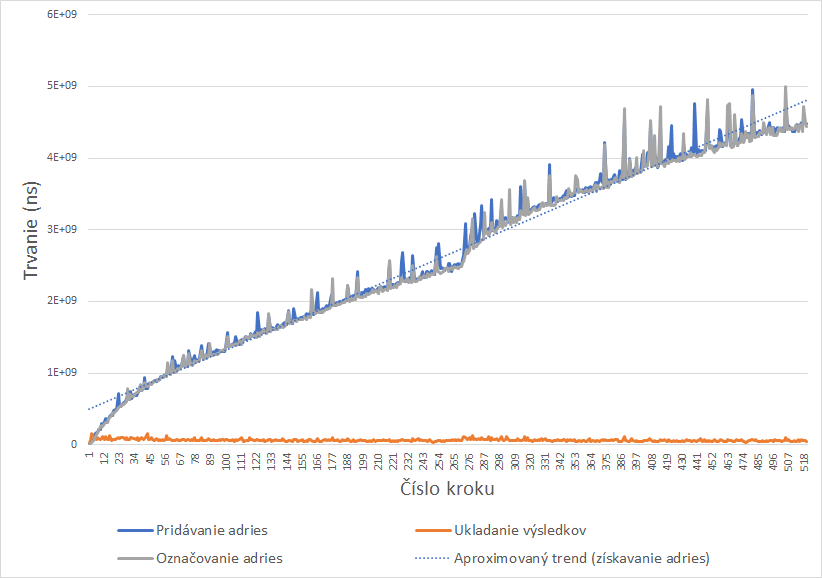
\includegraphics[width=1\textwidth]{figures/operationsTime.png}
    \caption{Graf závislosti dĺžky trvania operácii od počtu krokov\label{o:opTimes}}
\end{figure}

\begin{figure}[!ht]
    \centering
    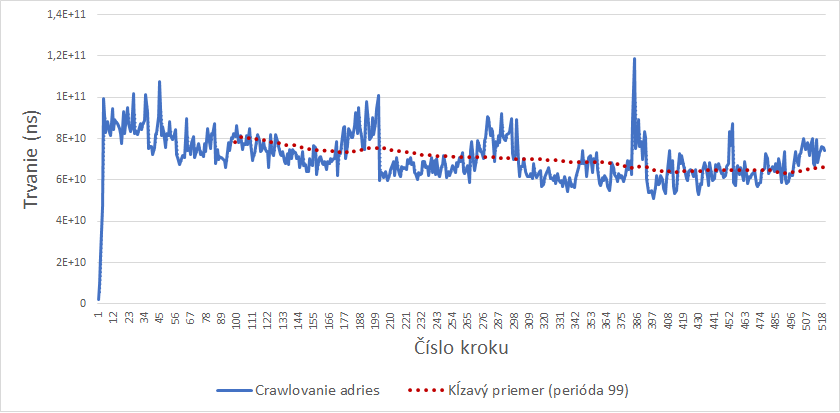
\includegraphics[width=1\textwidth]{figures/crawlTimeChart.png}
    \caption{Graf závislosti dĺžky trvania crawlovania od počtu krokov\label{o:crawlTimeChart}}
\end{figure}



\subsection{Počet adries na prejdenie} \label{c:addInteresting}
Očakávali sme prudký nárast adries na prejdenie v začiatku behu programu a následne stabilný lineárny pokles. To sa nepotvrdilo, na obrázku \ref{o:umSizeChart} vidíme, že v približnom strede behu, tento počet znovu začal prudko stúpať. 

Hypotézou bolo že, že sme objavili adresu odkazujúcu na časť webu, ktorá je málo odkazovaná zvyškom webu. Konkrétne v našom prípade sme prechádzali aj doménu https://primar.sme.sk, ale nemali sme ju v štartovacích adresách. Teda až prvým odkazom na túto doménu sme naštartovali jej objavovanie. 

Pre overenie sme pridali stránku z tejto domény ("https://primar.sme.sk/c/23168416/orl-lekar-mandle-su-ako-policajti-chrania-pred-zlom-ktore-by-nas-mohlo-ohrozit.html") do štartovacích adries a znova spustili crawler na 11 hodín. Systém a nastavenia zostali rovnaké. Výsledok sme ale dostali takmer totožný. Potvrdenie alebo vyvrátenie tejto hypotézy si vyžaduje hlbšiu analýzu.

\begin{figure}[!ht]
    \centering
    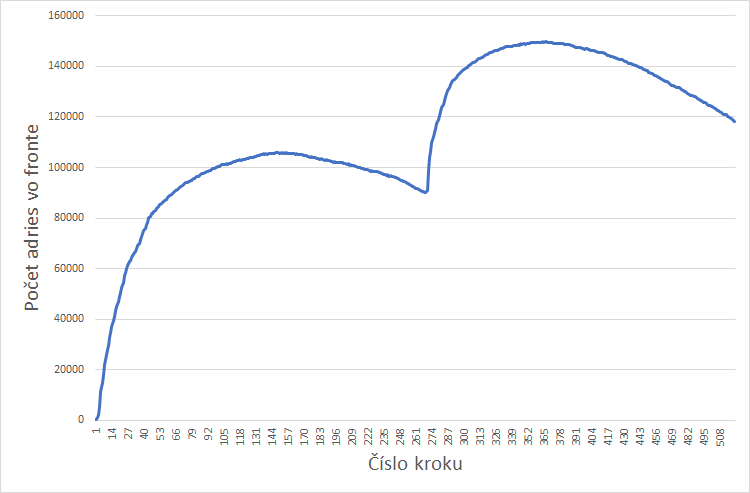
\includegraphics[width=.9\textwidth]{figures/umSizeChart.png}
    \caption{Graf závislosti počtu adries na prejdenie od počtu krokov\label{o:umSizeChart}}
\end{figure}





\section{Verifikovanie použiteľnosti dát}
Cieľom práce je navrhnutie a vytvorenie crawlera na zozbieranie dát zo spravodajských webov pre následnú analýzu v Apache Spark a ďalších produktoch v tomto ekosystéme. Touto podkapitolou overíme, či zozbierané dáta sú vo vhodnej forme a majú výpovednú hodnotu. 

Analytická časť celého procesu nie je cieľom tejto práce, preto na demonštráciu splnenia cieľa použijeme iba primitívnu analýzu analýza spätných odkazov, implementovanú kódom \ref{code:backlink} v Apache Spark. Pomocou nej sme identifikovali 1000 najviac odkazovaných článkov. Z tohto zoradenia vieme vyčítať najdôveryhodnejšie alebo aktuálne odporúčané články. Ukážka výstupu je na obrázku \ref{o:analRes}.

Dáta sme úspešne analyzovali a nevyskytli sa žiadne problémy. Myslíme, si že sú vhodné aj na zložitejšie analýzy. Preto považujeme tento cieľ práce za splnený.

\begin{lstlisting}[language=Scala,caption={Primitívna analýza spätných odkazov v Apache Spark}]
val df = spark.read
  .option("header", "true")
  .csv(files: _*)

val selectedDf = df
  .withColumn("child_urls", split(col("child_urls"), ", "))
  .filter(col("state") === "Crawled")
  .filter(col("article_text").isNotNull && col("article_text") =!= lit(""))

val explodedDf = selectedDf
  .withColumn("child_urls", explode(col("child_urls")))
  .filter(supportedDoms.foldLeft(lit(false)){case (acc, domStr) =>
    acc || col("child_urls").startsWith(domStr)})
  .dropDuplicates("url", "child_urls")

val groupedDf = explodedDf
  .groupBy("child_urls").count()
  .withColumnRenamed("count", "backlink_count")
  .withColumnRenamed("child_urls", "url")
  .orderBy(desc("backlink_count"))
  .select("backlink_count", "url")

groupedDf.limit(1000).write
  .option("header", "true")
  .format("csv").save(targetPath)
}
\end{lstlisting}\label{code:backlink}

\begin{figure}[!ht]
    \centering
    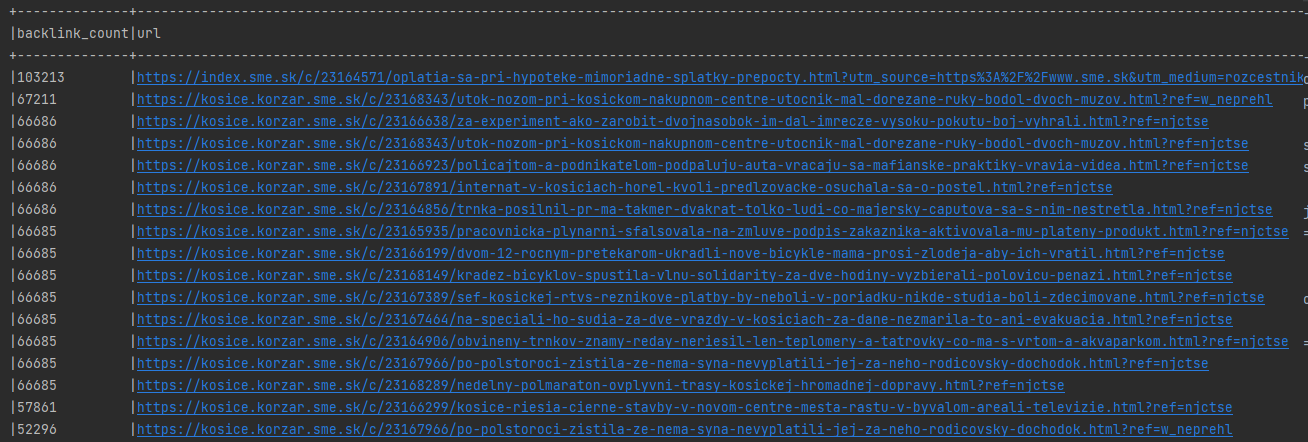
\includegraphics[width=1\textwidth]{figures/analExample.png}
    \caption{Ukážka výsledku analýzy\label{o:analRes}}
\end{figure}



\section{Splnenie požiadaviek}
Požiadavku na paralelizmus popísanú v podkapitole \ref{c:reqParalel} sme splnili. K stránkam pristupujeme paralelne a výkon sa neznižuje. Nemáme ani problém s blokovaním odpovedí serverom. Teda neprekročili sme maximálny počet dotazov. 

Požiadavku \ref{sec:reqFailRecovery} sme splnili čiastočne. Ukladáme stav Url Manažéra a výsledky crawlovania v každom kroku. Pri páde systému prídeme maximálne iba o jeden krok. Teda systém nie je odolný voči pádu operačného systému so stratou dát v súborovom systéme. Čo as ale podľa popisu požiadavky považuje za dostatočné. 

Pridaním nového extraktora pre novú doménu, implementujeme aj metódu isInDomain. Na jej základe sa filtrujú adresy pridávané do Url Manažéra. Týmto obmedzujeme doménu ako je v požiadavke \ref{c:reqDomain}.

Nie je potrebné nasadzovať databázu alebo iné externé systémy. Systém robí len to na čo bol nadizajnovaný a nie je zaťažený zbytočným balastom. Teda požiadavka \ref{c:reqKomplexity} je splnená. 

Ako je možné vidieť v tabuľke \ref{t:agrMer}, zbieranie dát nedosahuje ideálnu úspešnosť a v ďalších iteráciách je ju potrebné zlepšiť. Nepovažujeme to za chybu dizajnu, ale za nedostatočnú optimalizáciu extraktora. Zbierame požadované dáta, preto požiadavku \ref{c:reqData} považujeme za splnenú. 
